\documentclass{beamer}
\usetheme{Copenhagen}

% This is for handouts. uncomment if you want. put handout in document class
%\usepackage{pgfpages}
%\pgfpagesuselayout{4 on 1}[a4paper, border shrink=5mm, landscape]

\usepackage{amsmath,cancel,multicol}

\setbeamertemplate{navigation symbols}{}
\setbeamertemplate{headline}{}

\newcommand\blfootnote[1]{%
	\begingroup
	\renewcommand\thefootnote{}\footnote{#1}%
	\addtocounter{footnote}{-1}%
	\endgroup
}

\title{Academic Review - Physics}
\author{Dinan Mariano}
\institute{UP Mindoreños}
\date{January 2024}

\AtBeginSection[]{
	\begin{frame}
		\vfill
		\centering
		\begin{beamercolorbox}[sep=8pt,center,shadow=true,rounded=true]{title}
			\usebeamerfont{title}\insertsectionhead\par%
		\end{beamercolorbox}
		\vfill
	\end{frame}
}


%-------------------------END OF PREAMBLE------------------------------


\begin{document}
	
	
\begin{frame}
    \maketitle
\end{frame}

\begin{frame}{Topics}
	\begin{columns}
		\column{0.5\textwidth}
		\tableofcontents[sections={1-2}]
		\column{0.5\textwidth}
		\tableofcontents[sections={3-5}]
	\end{columns}
\end{frame}

%-------------------------------INTRO-----------------------------------

\begin{frame}{Nobel and Ig Nobel Prizes}
	2023 Nobel Prize of Physics - for experimental methods that generate attosecond pulses of light for the study of electron dynamics in matter\\~\\
	\uncover<2-> {
	\begin{block}{Ig Nobel Prize}
		Honor "achievements that first make people laugh and then make them think."
	\end{block}}
	
	\uncover<3>{2023 Ig Nobel Prize of Education - for methodically studying the boredom of teachers and students}
\end{frame}
\section{Scalar and Vector}

\subsection{Scalar and Vector}

\begin{frame}
	\begin{columns}
		\column{0.5\textwidth} \textbf{Scalar Quantity} - a quantity which is expressed by magnitude only \\
		\begin{example}
			Mass \\
			Time \\
			Temperature \\
			Area \\
			Distance 
		\end{example}
		\column{0.5\textwidth} \textbf{Vector Quantity} - a quantity which is expressed by magnitude and direction \\
		\begin{example}
			Force \\
			Velocity \\
			Weight \\
			Acceleration \\
			Displacement
		\end{example}
	\end{columns}
\end{frame}

\begin{frame}{Quiz}
		
		\begin{columns}
			\column{0.4\textwidth}
			\begin{itemize}
				\item 5 m
				\item 30 m/sec, East
				\item 5 km, North
				\item 20 degrees Celcius
				\item 1 GB
				\item 4000 calories
			\end{itemize}
			\column{0.6\textwidth}
			\begin{itemize}
				\item[--]<2-> Scalar
				\item[--]<3-> Vector
				\item[--]<4-> Vector
				\item[--]<5-> Scalar
				\item[--]<6-> Scalar
				\item[--]<7-> Scalar
			\end{itemize}
		\end{columns}
\end{frame}


%---------------------------RESULTANT VECTOR----------------------------------


\subsection{Resultant Vector}

\begin{frame}{Resultant Vector}
	
	\begin{definition}
		Sum of two or more vectors which will give the same effect as the original vectors
	\end{definition}
\end{frame}


\begin{frame}{Process of finding the Resultant Vector}
	
	\begin{enumerate}
		\item Addition/Subtraction
		\item Pythagorean Theorem
		\item Component Method
	\end{enumerate}
	
\end{frame}

\begin{frame}{Addition/Subtraction}
	\begin{columns}
		\column{0.5\textwidth}
		Can only be used on 1D vectors \\ (same direction)\\~\\
		\uncover<2-> {What if we encounter more complicated vectors?\\
		\begin{center}
			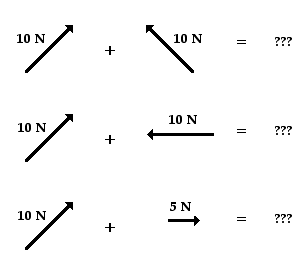
\includegraphics[scale=0.4]{compvec.png}
		\end{center}}
		\column{0.5\textwidth}
		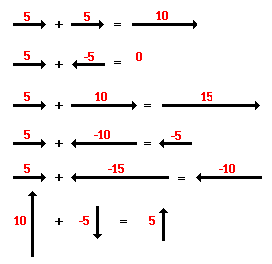
\includegraphics[scale=0.5]{vectoradd.png}
	\end{columns}
	
\end{frame}

\begin{frame}{Pythagorean Theorem}
	Pythagorean Theorem
	\begin{equation}
		 a^2 + b^2 = c^2
	\end{equation}
	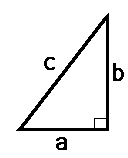
\includegraphics[scale=0.3]{pytha.png}  \uncover<2>{\alert{only use pythagorean theorem on perpendicular vectors!}}\\
	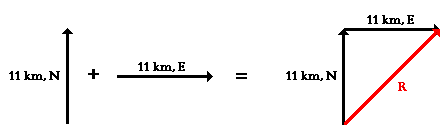
\includegraphics[scale=0.3]{pythaexample.png}
	\centering 
	\begin{align*}
		11^2 + 11^2 &= R^2\\
		242 &= R^2\\
		15.6 &= R
	\end{align*}
	
\end{frame}

\begin{frame}{Component Method}
	\begin{example}
		An airplane flies in a northeasterly direction at 100 km/h, at the same time there is a wind blowing at 20 km/h to the northwest. What is the resultant velocity of the plane?
	\end{example}
	X-components:
	\begin{align*}
		V_{xplane} &= V_{plane} \cos 45^\circ \\
		&= 70.71 \text{ km/h}	\\
		V_{xwind} &= -V_{wind}  \cos 45^\circ \\
		&= -14.14 \text{ km/h}
	\end{align*}
	\blfootnote{$V_{xwind}$ can be equal to $V_{wind} \cos 135^\circ$ with the same answer}
\end{frame}

\begin{frame}{Component Method (cont.)}
	Y-compoments:
	\begin{align*}
		V_{yplane} &= V_{plane} \sin 45^\circ \\
		&= 70.71 \text{ km/h} \\
		V_{ywind} &= V_{wind}  \sin 45^\circ \\
		&= 14.14 \text{ km/h}
	\end{align*}

\end{frame}

\begin{frame}{Component Method (cont.)}

	Resultant Velocity
	\begin{align*}
		V_x &= V_{xplane} + V_{xwind} \\
		&= 70.71 - 14.14 \\
		& = 56.57 \text{ km/h} \\
		V_y &= V_{yplane} + V_{ywind} \\
		&= 70.71 + 14.14 \\
		&= 84.85 \text{ km/h}\\
		R &= \sqrt{56.57^2 + 84.85^2} \\
		R &= 101.978857613  \text{ km/h}\\
		\theta &= \arctan{\frac{84.85}{56.57}} \\
		\theta &= 56.31^\circ
	\end{align*}
\end{frame}


%----------------------------------MECHANICS--------------------------------


\section{Mechanics}

\begin{frame}{Motion}
	\begin{definition}
		Change in position of a object relative to other objects that are considered at rest
	\end{definition}
	\vfil
	\begin{itemize}
		\item Distance vs. Displacement
		\item Speed vs. Velocity
		\item Acceleration
		\item Uniform Motion
		\item Uniformly Accelerated Rectilinear Motion (UARM)
		\item Projectile Motion
	\end{itemize}
\end{frame}


%----------------------------DISTANCE AND DISPLACEMENT----------------------


\subsection{Distance and Displacement}

\begin{frame}{Distance and Displacement}
	\begin{block}{Distance}
		Scalar quantity that refers to "how much ground an object has covered" during its motion.
	\end{block}
	\begin{block}{Displacement}
		Vector quantity that refers to "how far out of place an object is"; it is the object's overall change in position.
	\end{block}
	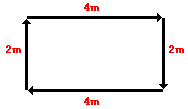
\includegraphics[scale=0.6]{distancedisp.png} \centering
\end{frame}

\begin{frame}{Quick Quiz}
	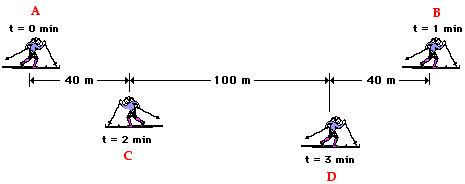
\includegraphics[scale=0.4]{distancedispquiz.png}\centering \\
	\uncover<2->{
		Distance
		\begin{align*}
			A \rightarrow B &= 180 \text{m} \\
			B \rightarrow C &= 140 \text{m} \\
			C \rightarrow D &= 100 \text{m} \\
			A \rightarrow D &= 420 \text{m} \\
		\end{align*}}
	\uncover<3->{
	Displacement
		\begin{equation*}
			A \rightarrow D = 140 \text{m, to the right}
		\end{equation*}}
	
\end{frame}


%---------------------------------SPEED VS. VELOCITY---------------------------


\subsection{Speed and Velocity}

\begin{frame}{Speed and Velocity}
	\begin{block}{Speed}
		Scalar quantity that refers to "how fast an object is moving."
	\end{block}
	\begin{block}{Velocity}
		Vector quantity that refers to "the rate at which an object changes its position."
	\end{block}
\end{frame}

\begin{frame}{Speed and Velocity}
	\textbf{Average Speed}
	\begin{equation}
		\text{Average Speed} = \frac{\text{Distance Traveled}}{\text{Time of Travel}}
	\end{equation}
	\textbf{Average Velocity}
	\begin{equation}
		\text{Average Velocity} = \frac{\text{displacement}}{\text{time}}
	\end{equation} \\~\\
	\textbf{Instantaneous Speed} - the speed at any given instant in time \\
	\textbf{Average Speed} - the average of all instantaneous speeds; found simply by a distance/time ratio
\end{frame}

\begin{frame}{Quick Quiz}
	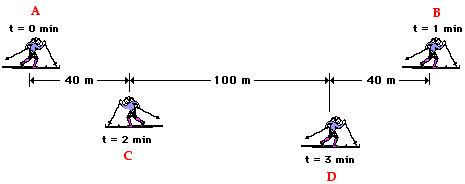
\includegraphics[scale=0.5]{distancedispquiz.png}\centering \\
	Average Speed
	\pause
	$$ \frac{420\text{m}}{3\text{min}} = 140\text{m/min}$$
	\pause
	Average Velocity
	\pause
	$$ \frac{140\text{m}}{3\text{m}} = 46.7\text{m/min, to the right}$$
\end{frame}


%-----------------------------------ACCELERATION-------------------------------

\subsection{Acceleration}

\begin{frame}{Acceleration}
	\begin{block}{Acceleration}
		Vector quantity that is defined as the rate at which an object changes its velocity. Anytime an object's velocity is changing, the object is said to be accelerating; it has an acceleration.
	\end{block}
\end{frame}

\begin{frame}{Graphs relating Displacement, Velocity, and Acceleration}
	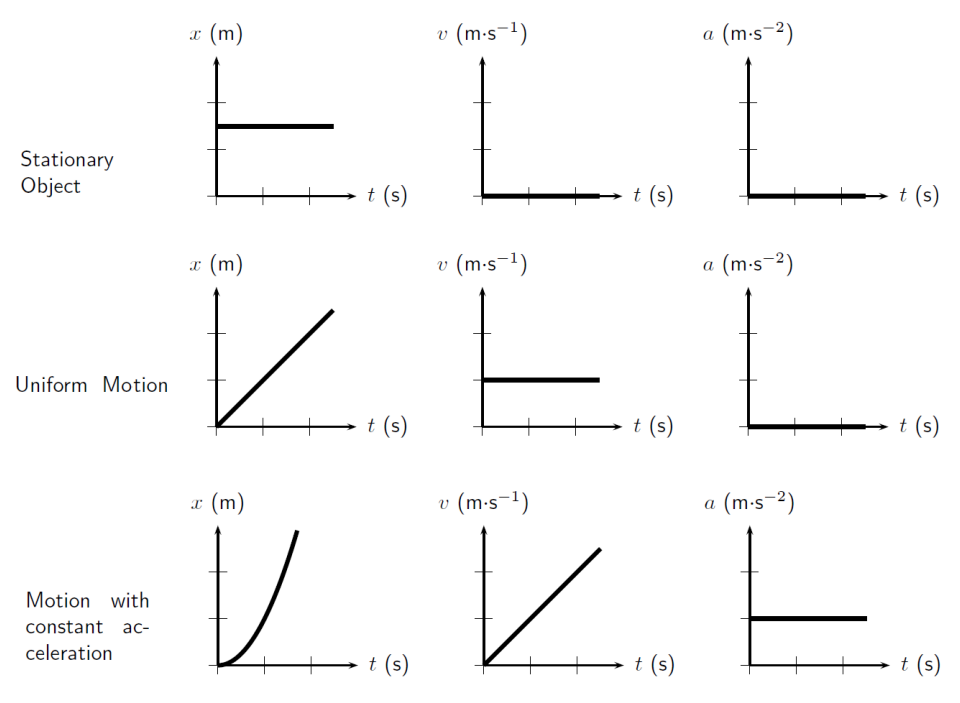
\includegraphics[scale=0.25]{graph.png}\centering
\end{frame}


\subsection{Uniform Motion}

\begin{frame}{Uniform Motion}
	\begin{block}{Uniform Motion}
		Motion with constant velocity
	\end{block}
	\begin{example}
		What is the displacement of a car moving at a constant velocity of 20m/s after 2 seconds? \\
		Given:
		\begin{align*}
			v &= 20 m/s \\
			t &= 2s
		\end{align*}
		Find $ \Delta x$ \\~\\
	\end{example}
\end{frame}

\begin{frame}{Uniform Motion (cont.)}
	\begin{example}
		Solution:
		\begin{align*}
			\onslide<2->{\Delta x &= vt} \\
			\onslide<3->{\Delta x &= 20\text{m/s} \cdot 2\text{s}} \\
			\onslide<4->{\Delta x &= 40 \text{m}}
		\end{align*}
	\end{example}
\end{frame}


\subsection{Uniformly Accelerated Rectilinear Motion}

\begin{frame}{Uniformly Accelerated Rectilinear Motion (UARM)}
	\begin{block}{UARM}
		Motion with constant acceleration
	\end{block}
	
	\begin{columns}
		\column{0.5\columnwidth}
		\begin{align}
			v_f &= v_0 + at \\
			x &= x_0 + v_0t + \frac{at^2}{2} \\
			v_f^2&=v_0^2 + 2a\Delta x\\
			\Delta x &=  \frac{(v_f+v_0)t}{2}
		\end{align}
		\column{0.5\columnwidth}
		Where:
		\begin{align*}
			v_f &= \text{ final velocity}\\
			v_0 &= \text{ initial velocity}\\
			a &= \text{ acceleration}\\
			t &= \text{ time}\\
			x &= \text{ final position}\\
			x_0 &= \text{ initial position}\\
			\Delta x &= x - x_0, \text{ displacement}
		\end{align*}
	\end{columns}
\end{frame}

\begin{frame}{UARM (cont.)}
	\begin{block}{Problem-Solving Strategy}
		\begin{enumerate}
			\item Construct an informative diagram of the physical situation.
			\item Identify and list the given information in variable form.
			\item Identify and list the unknown information in variable form.
			\item Identify and list the equation that will be used to determine unknown information from known information.
			\item Substitute known values into the equation and use appropriate algebraic steps to solve for the unknown information.
			\item Check your answer to insure that it is reasonable and mathematically correct.
		\end{enumerate}
	\end{block}
\end{frame}

\begin{frame}{UARM (cont.)}
	\begin{example}
		Vhonne is approaching a stoplight moving with a velocity of +30.0 m/s. The light turns yellow, and Vhonne applies the brakes and skids to a stop. If Ima's acceleration is -8.00 m/s$^2$, then determine the displacement of the car during the skidding process. (Note that the direction of the velocity and the acceleration vectors are denoted by a + and a - sign.)\\~\\
		
		\uncover<2>{We'll use Equation 6 $$v_f^2 = v_0^2 + 2ax$$}
	\end{example}
\end{frame}

\begin{frame}{UARM (cont.)}
	\begin{example}
		\begin{flalign*}
			\text{Given:}\\
			v_0 &= +30.0 \text{m/s}&&\\
			v_f &= 0 \text{m/s}&&\\
			a &= -8.00 \text{m/s}^2&&\\
			\text{Find:}\\
			x &= \text{ ?}&&
		\end{flalign*}
		\\~\\
	\end{example}
	
\end{frame}

\begin{frame}{UARM (cont.)}
	\begin{example}
		\begin{align*}
			v_f^2 &= v_0^2 + 2ax\\
			\onslide<2->{(0 \text{m/s})^2 &= (30.0 \text{m/s})^2 + 2 \cdot (-8.00 \text{m/s}^2) \cdot x }\\
			\onslide<3->{0 \text{m}^2/\text{s}^2 &= 900 \text{m}^2/\text{s}^2 + (-16.0 \text{m/s}^2) \cdot x}\\
			\onslide<4->{(16.0\text{m/s}^2) \cdot x &= 900 \text{m}^2/\text{s}^2 -0\text{m}^2/\text{s}^2}\\
			\onslide<5->{d &= \frac{900 \text{m}^2/\text{s}^2}{16.0\text{m/s}^2}}\\
			\onslide<6->{\therefore d &= 56.3 \text{m}}
		\end{align*}
	\end{example}
\end{frame}

\begin{frame}{UARM (cont.)}
	\begin{example}
		Annjo is waiting at a stoplight. When it finally turns green, Ben accelerated from rest at a rate of a 6.00 m/s$^2$ for a time of 4.10 seconds. Determine the displacement of Annjo's car during this time period. \\~\\
		
		\uncover<2>{We'll use Equation 5 $$ x = x_0 + v_0t + \frac{at^2}{2} $$}
	\end{example}
\end{frame}

\begin{frame}{UARM (cont.)}
\begin{example}
	\begin{flalign*}
		\text{Given:}\\
		v_0 &= 0 \text{m/s}&&\\
		t &= 4.10 \text{s}&&\\
		a &= 6.00 \text{m/s}^2 &&\\
		\text{Find:}\\
		x &= \text{ ?}
	\end{flalign*}
\end{example}
\end{frame}

\begin{frame}{UARM (cont.)}
	\begin{example}
		\begin{align*}
			x &= x_0 + v_0t + \frac{at^2}{2}\\
			\onslide<2->{x &= 0 \text{m/s} \cdot 4.1 \text{s} + \frac{6.00 \text{m/s}^2 \cdot 4.10 \text{s}^2}{2}} \\
			\onslide<3->{x &= 0 \text{m} + 50.43 \text{m}}\\
			\onslide<4->{\therefore x &= 50.4 \text{m}}	
		\end{align*}
	\end{example}
\end{frame}


%--------------------------FREE FALL------------------------------------
\begin{frame}{Free Fall}
	\begin{itemize}
		\item[--] example of uniform accelerated motion
		\item[--] one dimensional motion where the moving object is only under the influence of gravity
		\item[--] gravitational acceleration is equal to $-9.8 \text{m/s}^2$
	\end{itemize}
	
	\begin{block}{Free fall equations}
		\begin{align*}
		v_f &= v_0 + gt \\
		y &= y_0 + v_0t + \frac{gt^2}{2} \\
		v_f^2&=v_0^2 + 2g\Delta y\\
		\Delta y &=  \frac{(v_f+v_0)t}{2}\\
	\end{align*}
	\end{block}
\end{frame}

\begin{frame}{Free Fall (cont.)}
	\begin{example}
		A ball is dropped from a building without an initial velocity. Find the velocity of the ball after 5 seconds.
		
		\begin{flalign*}
			\text{Given:}\\
			t &= 5 \text{s}&&\\
			v_0 &= 0&&\\
			\text{Find:}\\
			v_f &= \text{ ?}
		\end{flalign*}
	\end{example}
\end{frame}

\begin{frame}{Free Fall (cont.)}
	\begin{example}
		\begin{flalign*}
			v_f &= v_0 + gt\\
			\onslide<2->{v_f &= 0 + (-9.8\text{m/s}^2)5\text{s}}\\
			\onslide<3->{\therefore v_f &= -49\text{m/s}}
		\end{flalign*}
	\end{example}
\end{frame}


\begin{frame}{Free Fall (cont.)}
	\begin{example}
		A mango falls from a tree. How far does it fall after 0.5 seconds?
		\begin{flalign*}
			\text{Given:}\\
			t &= 0.5 \text{s}&&\\
			v_0 &= 0&&\\
			\text{Find:}\\
			\Delta y &= \text{ ?}
		\end{flalign*}
	\end{example}
\end{frame}

\begin{frame}{Free Fall (cont.)}
	\begin{example}
		\begin{flalign*}
			\Delta y &= v_0t + \frac{gt^2}{2}\\
			\onslide<2->{\Delta y &= 0 + \frac{(-9.8 \text{m/s}^2)(0.5\text{s})^2}{2}}\\
			\onslide<3->{\Delta y &= \frac{(-9.8 \text{m/s}^2)(0.25\text{s}^2)}{2}}\\
			\onslide<4->{\therefore \Delta y &= -1.225\text{m}}
		\end{flalign*}
	\end{example}
\end{frame}


%---------------------------PROJECTILE MOTION-------------------------------


\subsection{Projectile Motion}

\begin{frame}{Projectile Motion}
	\begin{block}{Projectile Motion}
		- motion of an object that is projected into the air and acted upon by the gravitational force of the earth \alert{only}\\
		- a combination of an uniform motion and free fall
	\end{block}
	\begin{block}{Projectile}
		an object in the air that is allowed to move freely and is influenced \alert{only} by gravity
	\end{block}
	\begin{block}{Terms}
		Range - horizontal distance covered by a projectile\\
		Time of flight - time in which the projectile is up in the air\\
		Trajectory - curve traced by the path of the projectile\\ 
	\end{block}
\end{frame}

\begin{frame}{Projectile Motion (cont.)}
	\begin{block}{Conditions of Projectile Motion throughout the flight}
		\begin{itemize}
			\item Neglect the effect of air resistance to the projectile
			\item The horizontal and vertical motions are independent of each other. Separate the displacement and velocity to its x and y components
		\end{itemize}
	\end{block}
\end{frame}

\begin{frame}{Projectile Motion (cont.)}
	\only<1>{\begin{block}{Along the horizontal}
		\begin{itemize}
			\item the x component of the velocity is constant throughout the flight
			\item the horizontal displacement x, follows uniform motion
			\item formula along the horizontal is the same as uniform motion
		\end{itemize}
	\end{block}}
\end{frame}

\begin{frame}{Projectile Motion (cont.)}
	\begin{block}{Along the vertical}
		\begin{itemize}
			\item the x component of the velocity acts as freefall and thus only affected by the gravitational acceleration
			\item the velocity's sign is positive for upward motion while for downward motion it is negative
			\item upon hitting the ground, its velocity is always equal to zero
			\item the time required for the projectile to reach its maximum height from initial position is equal to the time that the projectile will reach the final position
			\item formula along the vertical is the same as free fall
		\end{itemize}
	\end{block}
\end{frame}

\begin{frame}{Projectile Motion (cont.)}
	\begin{block}{When the vertical displacement is at its maximum height}
		\begin{itemize}
			\item the x component of the velocity is constant
			\item the y component of the velocity is equal to zero
			\item the acceleration is still equal to g, -9.8 m/s$^2$
		\end{itemize}
	\end{block}
\end{frame}

\begin{frame}{Projectile Motion (cont.)}
	\begin{example}
		A stone is thrown with an initial horizontal velocity of 10m/s from the top of a tower 200m high. What is the horizontal displacement of the stone after 2 seconds? When will it hit the ground? What is its speed just before it hits the ground?
		\begin{flalign*}
			\text{Given:}\\
			v_x &= 10\text{m/s}&&\\
			\Delta y &= 200\text{m}&&\\
			t &= 2\text{s}&&\\
			\text{Find:}\\
			\Delta x  &= \text{ }? \text{ at }t = 2\text{s}&&\\
			t &= \text{ }?&&\\
			v_f &= \text{ }?&&
		\end{flalign*}
	\end{example}
\end{frame}

\begin{frame}{Projectile Motion (cont.)}
	\begin{example}
		Solving for $\Delta x$, we can use $ \Delta x = vt$.\\
		$ \Delta x = (10\text{m/s})(2\text{s})$\\
		$\Delta x = 20\text{m} $\\~\\
		Solving for the time when it hits the ground,
		\begin{flalign*}
			\text{Given:}\\
			\Delta y &= 200\text{m}&&\\
			v_0 &= 0&&\\
			\text{Find:}\\
			t&= \text{ }?
		\end{flalign*}
		$$ y = y_0 + v_0t + \frac{gt^2}{2}$$
	\end{example}
\end{frame}

\begin{frame}{Projectile Motion (cont.)}
	\begin{example}
		\begin{flalign*}
			y &= y_0 + v_0t +\frac{gt^2}{2}&&\\
			0 &= 200 + \cancel{0t} + \frac{(9.8\text{m/s}^2) (t^2)}{2}&&\\
			\frac{(9.8\text{m/s}^2) (t^2)}{2} &= -200&&\\
			t &= \sqrt{\frac{2(-200\text{m})}{-9.8\text{m/s}^2}}&&\\
			\therefore t &= 6.39 \text{s}
		\end{flalign*}
	\end{example}
\end{frame}

\begin{frame}{Projectile Motion (cont.)}
	\begin{example}
		\begin{flalign*}
			\text{Solving for final velocity $v_f$:}\\
			v_f &= v_0 + gt&&\\
			v_f &= 0 + (-9.8\text{m/s}^2)(6.38\text{s})&&\\
			v_f &= -62.52 \text{m/s}
		\end{flalign*}
	\end{example}
\end{frame}


%----------------------------------NEWTON'S LAW----------------------------------


\section{Newton's Law of Motion}

\subsection{First Law of Motion}

\begin{frame}{Newton's Law of Motion}
	\begin{block}{First Law of Motion (Law of Inertia)}
		An object at rest stays at rest and an object in motion stays in motion with the same speed and in the same direction unless acted upon by an unbalanced force.
		
		\begin{itemize}
			\item Objects tend to "keep on doing what they're doing."
			\item The tendency to resist changes in their state of motion is \alert{inertia}
			\item Forces don't keep objects moving. Forces cause acceleration
			\item The more inertia the object has, the more mass that it has
			\item A more massive object has a greater tendency to resist changes in its state of motion
		\end{itemize}
	\end{block}
\end{frame}

\subsection{Second Law of Motion}

\begin{frame}{Newton's Law of Motion (cont.)}
	\begin{block}{Second Law of Motion (Law of Acceleration)}
		\begin{equation}
			F = ma
		\end{equation}
		Force and mass have opposite effect on acceleration. The more massive the object, the less is the acceleration. This means that acceleration is inversely proportional to the mass. \\~\\
		A greater force will result to greater acceleration. Force is directly proportional to the acceleration of an object. Again, Forces cause acceleration and not required to keep an object moving
	\end{block}
\end{frame}

\begin{frame}{Newton's Law of Motion (cont.)}
	\begin{example}
		Neglecting friction, what constant force will give a mass of 50kg an acceleration of 5m/s$^2$?
		\begin{flalign*}
			\text{Given:}\\
			m &= 50\text{kg}&&\\
			a &= 5\text{m/s}^2&&\\
			\text{Find }F\\
			\uncover<2->{\text{Solution:}\\
			F &= ma&&\\
			F &= (50\text{kg})(5\text{m/s}^2)&&\\	
			F &= 250 \text{kg m/s}^2 \text{ or } 250\text{N}&&}
		\end{flalign*}
	\end{example}
\end{frame}

\subsection{Third Law of Motion}

\begin{frame}{Newton's Law of Motion (cont.)}
	\begin{block}{Third Law of Motion (Law of action-reaction)}
		For every action, there is an equal and opposite reaction.
		\\~\\
		\only<2>{The statement means that in every interaction, there is a pair of forces acting on the two interacting objects. The size of the forces on the first object equals the size of the force on the second object. The direction of the force on the first object is opposite to the direction of the force on the second object. Forces always come in pairs - equal and opposite action-reaction force pairs. }
	\end{block}
\end{frame}

\section{Momentum and Impulse}

\subsection{Momentum}



\begin{frame} {Momentum and Impulse}
	\begin{block}{Momentum}
		Momentum is a physical quantity obtained when the mass of an object is multiplied to its velocity. It has the same direction as the velocity. This means that an object with large mass and velocity has high momentum. Accordingly, an object at rest has a momentum equal to zero.
		\begin{equation}
			p = mv
		\end{equation}
		Where: 
		\begin{align*}
			p &= \text{momentum}\\
			m &= \text{mass}\\
			v &= \text{velocity}
		\end{align*}
	\end{block}
\end{frame}

\begin{frame}{Momentum (cont.)}
	\begin{example}
		A truck full of sand with a mass of 40000 kg travels east with a velocity of 50 m/s. What is the truck's momentum?\\~\\
		Solving for $p$
		\begin{align*}
			p &= mv\\
			p &= 40000\text{kg} \cdot 50 \text{m/s}\\
			p &= 2000000 \text{kg }\cdot \text{m/s}
		\end{align*}
	\end{example}
\end{frame}

\subsection{Impulse}

\begin{frame}{Impulse}
	\begin{block}{Impulse}
		Impulse is a vector quantity that has the same direction as the force. It is equal to the product of force and time. It is also associated with the change of momentum.
		
		
	\end{block}
\end{frame}

\begin{frame}{Impulse (cont.)}
	\begin{block}{Impulse}
		\begin{align}
			J &= \Delta mv\\
			\frac{J}{\Delta t} &= \frac{\Delta mv}{\Delta t} = \frac{m \Delta v}{\Delta t} = ma = F\\
			J &= F\Delta t
		\end{align}
		\hfil Where:
		\begin{align*}
			J &= \text{impulse}\\
			F &= \text{force}\\
			\Delta t &= \text{change in time}\\
			m &=\text{mass}\\
			v &= \text{velocity}
		\end{align*}
	\end{block}
\end{frame}

\begin{frame}{Impulse (cont.)}
	\begin{example}
		A bat hits a baseball. The bat and the baseball remain in contact for 0.005 seconds. The 0.1 kg ball leaves the bat with a velocity of 100 m/s. What is the average force of the bat on the baseball
		\begin{flalign*}
			\text{Given:}\\
			t &= 0.005 \text{s}&&\\
			m &= 0.1 \text{kg}&&\\
			v &= 100 \text{m/s}\\
			\text{Find: }\\
			F &= \text{ }?
		\end{flalign*}
	\end{example}
\end{frame}

\begin{frame}{Impulse (cont.)}
	\begin{example}
		
		Solution:
		\begin{align*}
			F &= \frac{\Delta mv}{\Delta t}\\
			F &= \frac{0.1\text{kg} \cdot 100\text{m/s} - 0}{0.005\text{s}}\\
			F &= 2000 \text{N}
		\end{align*}
	\end{example}
\end{frame}

\section{Work, Energy, and Power}

\subsection{Work}

\begin{frame}
	\begin{block}{Work}
		The product of force and displacement
		\begin{equation}
			W = F \cdot \Delta x \cos \theta
		\end{equation}
		Where:
		\begin{align*}
			W &= \text{work}\\
			F &= \text{force}\\
			\Delta x &= displacement
		\end{align*}
		\alert{A force does no work if it is perpendicular to the displacement}
	\end{block}
\end{frame}

\begin{frame}{Work (cont.)}
	\begin{example}
		A 100 N block lies on a frictionless surface. A force of 20N was applied horizontally where the block had moved 5m. Find the work done by the force and weight of the block.
		
		\begin{flalign*}
			\text{Given:}\\
			W &= 100 \text{N} &&\\
			F &= 20 \text{N} &&\\
			\Delta x &= 5 \text{m}&&\\
			\text{Find:}\\
			W_{force} &= ?&&\\
			W_{weight} &= ?&&
		\end{flalign*}
	\end{example}
\end{frame}

\begin{frame}{Work (cont.)}
	\begin{example}
		Solution:
	\begin{align*}
		W &= F\cdot \Delta x \cos \theta\\
		W_{force} &= 20\text{N} \cdot \text{5m} \cos 0\\
		\therefore W_{force} &= 100 \text{Nm} = 100\text{Joules}\\~\\
		W_{weight} &= 100\text{N} \cdot 5 \text{m} \cos 90\\
		\therefore W_{weight} &= 0
	\end{align*}
	\end{example}
\end{frame}

\subsection{Energy}

\begin{frame}{Energy}
	\begin{block}{Energy}
		\begin{itemize}
			\item[--] capacity to do work
			\item[--] scalar quantity
		\end{itemize}
		Types of Mechanical Energy
		\begin{enumerate}
			\item Potential Energy - energy stored on an object due to its position
			\begin{itemize}
				\item Gravitational Potential Energy
				\begin{flalign}
					PE_{grav} &= mgh&&
				\end{flalign}
				\item Elastic Potential Energy - energy stored on an elastic material due to its stretching or compressing
				\begin{flalign}
					PE_{s} &= \frac{1}{2}k \Delta x^2&&
				\end{flalign}
			\end{itemize}
		\end{enumerate}
	\end{block}
\end{frame}

\begin{frame}{Energy (cont.)}
	\begin{block}{Energy}
		\begin{enumerate}
			\setcounter{enumi}{1}
			\item Kinetic Energy - energy of an object in motion
			\begin{flalign}
				KE &= \frac{1}{2}mv^2&&
			\end{flalign}
		\end{enumerate}
		Total Mechanical Energy
		\begin{flalign}
			TME &= PE + KE&&
		\end{flalign}
	\end{block}
\end{frame}

\subsection{Power}

\begin{frame}{Power}
	\begin{block}{Power}
		Power is the rate at which work is done
		\begin{align}
			P &= \frac{W}{t}\\
			P &= \frac{F\cdot \Delta x}{t} \notag \\
			P &= F \frac{\Delta x}{t} \notag \\
			P &= Fv
		\end{align}
	\end{block}
\end{frame}

\end{document}


% Todo:
% Examples for Energy and Power, Acceleration
% Mini quiz at the end for all topics
% (Optional) Put pauses for slides for it to have animation






